\documentclass{standalone}
\usepackage{tikz}
\usepackage{adjustbox}
\usepackage{helvet}  
\usepackage{sansmathfonts}  
\renewcommand{\familydefault}{\sfdefault}  
\usetikzlibrary{arrows.meta,calc,decorations.pathmorphing}
\usetikzlibrary{shapes.geometric, shapes.arrows}
\usepackage{xcolor}

\definecolor{color0000FF}{HTML}{0000FF}
\definecolor{colorADD8E6}{HTML}{ADD8E6}
\definecolor{colorFF0000}{HTML}{FF0000}
\definecolor{colorFFC0CB}{HTML}{FFC0CB}
\definecolor{color008000}{HTML}{008000}
\definecolor{color90EE90}{HTML}{90EE90}
\definecolor{colorFFA500}{HTML}{FFA500}
\definecolor{colorFFFF00}{HTML}{FFFF00}
\definecolor{color800080}{HTML}{800080}
\definecolor{colorE6E6FA}{HTML}{E6E6FA}
\definecolor{color000000}{HTML}{000000}
\definecolor{colorD3D3D3}{HTML}{D3D3D3}
\begin{document}
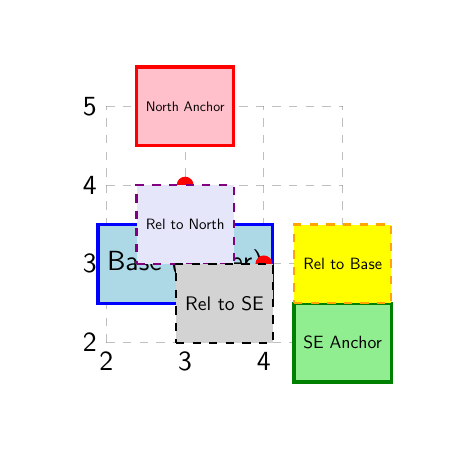
\begin{tikzpicture}
\useasboundingbox (1,1) rectangle (6,6);



\draw[dashed,gray,opacity=0.5] (2,2) -- (2,5);
\node[below] at (2,2) {2};
\draw[dashed,gray,opacity=0.5] (3,2) -- (3,5);
\node[below] at (3,2) {3};
\draw[dashed,gray,opacity=0.5] (4,2) -- (4,5);
\node[below] at (4,2) {4};
\draw[dashed,gray,opacity=0.5] (5,2) -- (5,5);
\node[below] at (5,2) {5};
\draw[dashed,gray,opacity=0.5] (2,2) -- (5,2);
\node[left] at (2,2) {2};
\draw[dashed,gray,opacity=0.5] (2,3) -- (5,3);
\node[left] at (2,3) {3};
\draw[dashed,gray,opacity=0.5] (2,4) -- (5,4);
\node[left] at (2,4) {4};
\draw[dashed,gray,opacity=0.5] (2,5) -- (5,5);
\node[left] at (2,5) {5};
\node[draw=color0000FF, fill=colorADD8E6, very thick, minimum width=2cm, minimum height=1cm] (base) at (3,3) {\adjustbox{max width=2cm, max height=1cm}{Base (center)}};
\node[draw=colorFF0000, fill=colorFFC0CB, very thick, minimum width=1cm, minimum height=1cm] (north_anchored) at (3,5) {\adjustbox{max width=1cm, max height=1cm}{North Anchor}};
\node[draw=color008000, fill=color90EE90, very thick, minimum width=1cm, minimum height=1cm] (south_east_anchored) at (5,2) {\adjustbox{max width=1cm, max height=1cm}{SE Anchor}};
\node[draw=colorFF0000, fill=colorFF0000, circle, inner sep=1pt, minimum width=0.2cm, minimum height=0.2cm] (base_east_marker) at (4,3) {};
\node[draw=colorFF0000, fill=colorFF0000, circle, inner sep=1pt, minimum width=0.2cm, minimum height=0.2cm] (north_south_marker) at (3,4) {};
\node[draw=colorFF0000, fill=colorFF0000, circle, inner sep=1pt, minimum width=0.2cm, minimum height=0.2cm] (se_west_marker) at (4,2.5) {};
\node[draw=colorFFA500, fill=colorFFFF00, dashed, thick, minimum width=1cm, minimum height=1cm] (rel_to_base) at (5,3) {\adjustbox{max width=1cm, max height=1cm}{Rel to Base}};
\node[draw=color800080, fill=colorE6E6FA, dashed, thick, minimum width=1cm, minimum height=1cm] (rel_to_north) at (3,3.5) {\adjustbox{max width=1cm, max height=1cm}{Rel to North}};
\node[draw=color000000, fill=colorD3D3D3, dashed, thick, minimum width=1cm, minimum height=1cm] (rel_to_se) at (3.5,2.5) {\adjustbox{max width=1cm, max height=1cm}{Rel to SE}};

\end{tikzpicture}
\end{document}